% !TEX program = pdflatex
% ============================================================
%  TEMPLATE APPUNTI
%  Compila con pdflatex (due passaggi per indice e riferimenti)
% ============================================================
\documentclass[11pt,a4paper,oneside]{book}

% ---------- Dati del documento (modifica qui) ----------------
\newcommand{\corso}{Laboratorio 1 ed Elementi di Computazione}
\newcommand{\sottotitolo}{Appunti delle lezioni}
\newcommand{\autore}{Cristiano Battini}
\newcommand{\universita}{Università di Pisa}
\newcommand{\annoaccademico}{Anno Accademico 2026/2027}

% ---------- Lingua e codifica --------------------------------
\usepackage[T1]{fontenc}
\usepackage[utf8]{inputenc}
\IfFileExists{italian.ldf}
  {\usepackage[italian]{babel}}
  {% ripiego se babel-italian non è installato
   \AtBeginDocument{%
     \renewcommand{\contentsname}{Indice}%
     \renewcommand{\chaptername}{Capitolo}%
     \renewcommand{\figurename}{Figura}%
     \renewcommand{\tablename}{Tabella}}}

% ---------- Font ---------------------------------------------
\usepackage[sc]{mathpazo}      % Palatino + matematica coordinata
\usepackage{courier}
\linespread{1.06}
\usepackage{microtype}

% ---------- Pagina -------------------------------------------
\usepackage[a4paper,top=2.8cm,bottom=3cm,inner=2.8cm,outer=2.8cm,
            headheight=15pt]{geometry}
\setlength{\parindent}{0pt}
\setlength{\parskip}{0.55em plus 0.1em minus 0.1em}

% ---------- Matematica ---------------------------------------
\usepackage{amsmath,amssymb,amsthm,mathtools,bm}
\usepackage{cancel}
\usepackage{siunitx}
\sisetup{output-decimal-marker={,},per-mode=symbol}

% ---------- Grafica, tabelle, liste --------------------------
\usepackage{graphicx}
\usepackage{booktabs,array}
\usepackage{enumitem}
\setlist{itemsep=0.2em,topsep=0.3em}
\usepackage{xcolor}
\usepackage{tikz}
\usetikzlibrary{decorations.pathreplacing}
\usepackage[most]{tcolorbox}

% ---------- Colori (volutamente pochi) -----------------------
\definecolor{filetto}{gray}{0.25}   % cornici e filetti
\definecolor{fondo}{gray}{0.955}    % fondo degli enunciati
\definecolor{grigio}{gray}{0.40}    % testo secondario
\definecolor{link}{HTML}{1A2F5A}    % collegamenti
% colori dei box (toni spenti)
\definecolor{cdef}{HTML}{1F3A5F}    % blu      – definizioni
\definecolor{cteo}{HTML}{6E2633}    % bordeaux – teoremi, proposizioni, lemmi, corollari
\definecolor{cese}{HTML}{2E5E4A}    % verde    – esempi, esercizi
\definecolor{coss}{HTML}{8A6A2A}    % ocra     – osservazioni, note
\definecolor{catt}{HTML}{9B2D20}    % rosso    – attenzione
\definecolor{cfor}{HTML}{3D3A6B}    % indaco   – formule, riquadri, riepilogo

% ---------- Collegamenti -------------------------------------
\usepackage[colorlinks=true,linkcolor=link,urlcolor=link,citecolor=link]{hyperref}

% ---------- Titoli di capitolo e sezione ---------------------
\usepackage{titlesec}
\titleformat{\chapter}[display]
  {\normalfont}
  {\large\scshape\lsstyle\MakeLowercase{\chaptertitlename}\ \thechapter}
  {8pt}
  {\Huge\bfseries}
  [{\vspace{8pt}\titlerule[0.6pt]}]
\titlespacing*{\chapter}{0pt}{0pt}{28pt}
\renewcommand{\thesection}{\arabic{section}}
\titleformat{\section}{\normalfont\LARGE\bfseries}{\thesection}{0.8em}{}[{\vspace{2pt}\titlerule[0.6pt]}]
\titlespacing*{\section}{0pt}{2.4em}{1em}
\titleformat{\subsection}{\normalfont\large\bfseries}{\thesubsection}{0.8em}{}
\titleformat{\subsubsection}{\normalfont\normalsize\bfseries\itshape}{\thesubsubsection}{0.8em}{}

% ---------- Intestazione e piè di pagina ---------------------
\usepackage{fancyhdr}
\pagestyle{fancy}
\fancyhf{}
\renewcommand{\chaptermark}[1]{\markboth{\thechapter.\ #1}{}}
\renewcommand{\sectionmark}[1]{\markright{\thesection.\ #1}}
\fancyhead[L]{\small\scshape\MakeLowercase{\corso}}
\fancyhead[R]{\small\itshape\nouppercase{\rightmark}}
\fancyfoot[C]{\small\thepage}
\renewcommand{\headrulewidth}{0.4pt}
\fancypagestyle{plain}{\fancyhf{}\renewcommand{\headrulewidth}{0pt}%
  \fancyfoot[C]{\small\thepage}}

% ============================================================
%  BOX
% ============================================================
% Stile comune: titolo in linea ("Teorema 1.2 (Titolo).")
\tcbset{
  base/.style={
    enhanced, breakable, sharp corners,
    colback=#1!5, colframe=#1, coltitle=#1,
    boxrule=0.5pt,
    left=9pt, right=9pt, top=7pt, bottom=7pt,
    before skip=1em, after skip=1em,
    fonttitle=\upshape\bfseries, description font=\upshape\mdseries,
    separator sign none, description delimiters parenthesis,
    detach title, before upper={{\color{#1}\tcbtitle.}\enspace}
  },
  % cornice completa: definizioni ed enunciati
  cornice/.style={base=#1},
  % solo filetto a sinistra: esempi, esercizi, osservazioni
  filetto/.style={base=#1, boxrule=0pt, leftrule=2pt,
    left=10pt, top=5pt, bottom=5pt}
}

% --- Box numerati:  \begin{definizione}{Titolo}{etichetta} ... \end{definizione}
%     Riferimento:   \ref{def:etichetta}   (titolo ed etichetta possono essere vuoti)
\newtcbtheorem[number within=section]{definizione}{Definizione}{cornice=cdef}{def}
\newtcbtheorem[use counter from=definizione]{teorema}{Teorema}{cornice=cteo, fontupper=\itshape}{teo}
\newtcbtheorem[use counter from=definizione]{proposizione}{Proposizione}{cornice=cteo, fontupper=\itshape}{prop}
\newtcbtheorem[use counter from=definizione]{lemma}{Lemma}{cornice=cteo, fontupper=\itshape}{lem}
\newtcbtheorem[use counter from=definizione]{corollario}{Corollario}{cornice=cteo, fontupper=\itshape}{cor}
\newtcbtheorem[number within=section]{esempio}{Esempio}{filetto=cese}{es}
\newtcbtheorem[number within=section]{esercizio}{Esercizio}{filetto=cese}{ex}

% --- Box non numerati:  \begin{osservazione}[Titolo opzionale] ... \end{osservazione}
\newcommand{\titolobox}[3]{{\color{#1}\textbf{#2}\ifx\relax#3\relax\else\ (#3)\fi.}\enspace}
\newtcolorbox{osservazione}[1][]{filetto=coss, before upper={\titolobox{coss}{Osservazione}{#1}}}
\newtcolorbox{nota}[1][]{filetto=coss, before upper={\titolobox{coss}{Nota}{#1}}}
\newtcolorbox{attenzione}[1][]{cornice=catt, before upper={\titolobox{catt}{Attenzione}{#1}}}
\newtcolorbox{riquadro}[1]{cornice=cfor, before upper={\titolobox{cfor}{#1}{}}}  % titolo libero

% --- Dimostrazione (stile classico, con quadratino di chiusura)
\newenvironment{dimostrazione}[1][]
  {\begin{proof}[Dimostrazione\ifx\relax#1\relax\else\ (#1)\fi]}
  {\end{proof}}

% --- Formula in cornice:  \begin{formulabox} ... \end{formulabox}
\newtcolorbox{formulabox}{
  enhanced, sharp corners, colback=cfor!5, colframe=cfor, boxrule=0.5pt,
  left=8pt, right=8pt, top=0pt, bottom=4pt, before skip=1em, after skip=1em
}
% --- Cornice attorno a una singola espressione dentro un'equazione: \evid{...}
\newcommand{\evid}[1]{{\setlength{\fboxsep}{4pt}\fcolorbox{cfor}{cfor!5}{$\displaystyle #1$}}}

% --- Riepilogo di fine capitolo
\newtcolorbox{riepilogo}[1][Riepilogo]{
  enhanced, breakable, sharp corners, colback=cfor!5, colframe=cfor,
  boxrule=0pt, toprule=0.8pt, bottomrule=0.8pt,
  left=9pt, right=9pt, top=7pt, bottom=7pt, before skip=1.4em, after skip=1em,
  before upper={{\color{cfor}\bfseries #1}\par\smallskip}
}

% ---------- Elementi accessori -------------------------------
% Data della lezione: \lezione{4 ottobre 2026}
\newcommand{\lezione}[1]{\par\medskip\noindent
  {\small\itshape\color{grigio}Lezione del #1}\par\smallskip}
% Separatore
\newcommand{\separatore}{\par\bigskip\noindent\hfil\rule{0.25\textwidth}{0.4pt}\par\bigskip}
% Annotazione a margine degli appunti (colonna "Spunti e domande")
\newtcolorbox{spunto}{filetto=coss, before upper={\titolobox{coss}{Spunti e domande}{}}}
% Annotazione secondaria (scritta in grigio negli appunti)
\newcommand{\grigio}[1]{{\color{grigio}#1}}
% Frecce e numeri cerchiati
\newcommand{\fr}{\ensuremath{\rightarrow}}
\newcommand{\giu}{\ensuremath{\hookrightarrow}}
\newcommand{\cerchio}[1]{\tikz[baseline=(c.base)]\node[draw,circle,inner sep=1.2pt,font=\small] (c) {#1};}
% Termine chiave
\newcommand{\chiave}[1]{\textbf{#1}}

% ---------- Scorciatoie matematiche --------------------------
\newcommand{\N}{\mathbb{N}}
\newcommand{\Z}{\mathbb{Z}}
\newcommand{\Q}{\mathbb{Q}}
\newcommand{\R}{\mathbb{R}}
\newcommand{\C}{\mathbb{C}}
\newcommand{\dd}{\mathop{}\!\mathrm{d}}
\newcommand{\vett}[1]{\vec{#1}}
\DeclarePairedDelimiter{\abs}{\lvert}{\rvert}
\DeclarePairedDelimiter{\norma}{\lVert}{\rVert}

% ============================================================
\begin{document}

% ---------- Frontespizio -------------------------------------
\begin{titlepage}
\centering
{\large\scshape\lsstyle\MakeLowercase{\universita}\par}
\vspace{0.3cm}
{\annoaccademico\par}
\vspace{5.5cm}
\rule{\textwidth}{0.8pt}\par
\vspace{0.6cm}
{\fontsize{28}{34}\selectfont\bfseries\corso\par}
\vspace{0.5cm}
{\Large\itshape\sottotitolo\par}
\vspace{0.5cm}
\rule{\textwidth}{0.8pt}\par
\vspace{2.5cm}
{\small\scshape autore}\\[3pt]\autore\par
\vfill
{\small Ultimo aggiornamento: \today\par}
\end{titlepage}

\frontmatter
\tableofcontents
\mainmatter
\setcounter{secnumdepth}{1}

% ============================================================
%  APPUNTI
% ============================================================

\section{Misura}
\lezione{14/09/26}

Met.\ scientifico
\begin{enumerate}[label=\arabic* --]
  \item Osservazione
  \item Modellizzazione \fr\ Teoria predittiva
  \item MISURA
  \item Compatibilità \fr\ Misura $\leftrightarrow$ Teoria?
\end{enumerate}

\chiave{MISURA} \fr\ compromesso tra precisione ed errore: qual'è più grande?

\giu\ è \chiave{sempre un intervallo} \qquad es.\ misura: $11 < l < 12$ \quad non si sa precisamente il valore

Come si scrive?
\[
  x = \hat{x} \pm \Delta x \ \ \text{unità di misura}
\]
\begin{itemize}
  \item $x$: Misurando
  \item $\hat{x}$: Valore centrale
  \item $\Delta x$: \chiave{Incertezza}
\end{itemize}

\begin{definizione}{Errore massimo}{erroremassimo}
$\Delta x$: \chiave{errore massimo} \fr\ Intervallo con prob $100\%$ di contenere il misurando
\[
  \Delta x = \frac{x_{\max} - x_{\min}}{2}
\]
\grigio{Non è giusto da usare: troppo grande}
\end{definizione}

Cosa si usa?

\begin{definizione}
{Errore statistico}{errorestatistico}
$\sigma_x$: \chiave{errore statistico}
\[
  x = \hat{x} \pm \sigma_x
\]
\[
  [\,\hat{x} + \sigma_x \,;\, \hat{x} - \sigma_x\,] \quad \text{prob} < 1 \ \text{contenere } x
\]
prob $< 100\%$ \fr\ Si definisce con $\sigma_x$
\end{definizione}

\begin{definizione}
{Errore relativo}{errorelinguaggio}
$\varepsilon_r$: \chiave{errore relativo}
\[
  \varepsilon_r = \frac{\sigma_x}{\abs{\hat{x}}}
\]
\end{definizione}

% ------------------------------------------------------------
\newpage
\section{Unità di misura}

es.\quad $L = (2.3 \pm 0.1)\ \mathrm{m}$ \fr\ uguale per tutti

\begin{spunto}
A cosa serve? Definisce la misura
\end{spunto}

SI \fr\ Sistema intern.\ di misura. Dà le definizioni

\begin{attenzione}
Come si definiscono le grandezze fondamentali?

\giu\ \chiave{Costanti fondamentali}
\end{attenzione}

\subsection*{Analisi dimensionale}
\[
  A = B
\]

\begin{esempio}{}{}
\leavevmode\par
\begin{minipage}[c]{0.38\linewidth}
\centering
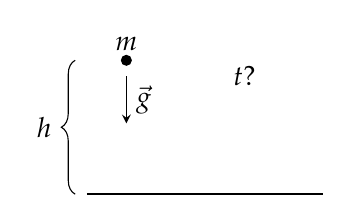
\begin{tikzpicture}[>=stealth]
  \draw[thick] (0,0) -- (3,0);
  \draw[decorate,decoration={brace,amplitude=5pt}] (-0.15,0) -- (-0.15,1.7) node[midway,left=5pt] {$h$};
  \fill (0.5,1.7) circle (2pt) node[above] {$m$};
  \draw[->] (0.5,1.5) -- (0.5,0.9) node[midway,right] {$\vec{g}$};
  \node at (2,1.5) {$t$?};
\end{tikzpicture}
\end{minipage}\hfill
\begin{minipage}[c]{0.55\linewidth}
-- Da cosa dipende?
\begin{itemize}
  \item $h$
  \item $g$
  \item $m$
\end{itemize}
\end{minipage}
\[
  t = c\, h^{\alpha} g^{\beta} m^{\gamma} \qquad (c\text{: costante adim.})
\]
Dimensioni:
\[
  \left.
  \begin{aligned}
    [t] &= T \\
    [h] &= L \\
    [g] &= L \cdot T^{-2} \\
    [m] &= M
  \end{aligned}
  \right\}
\]
\[
  \to\
  \begin{aligned}
    [t] &= [c]\,[h]^{\alpha}\,[g]^{\beta}\,[m]^{\gamma} \qquad ([c] = 1)\\
    T &= 1 \cdot L^{\alpha} \,(L \cdot T^{-2})^{\beta}\, M^{\gamma} \\
    T^{1} &= L^{\alpha+\beta} \cdot T^{-2\beta} \cdot M^{\gamma}
  \end{aligned}
\]
\[
  \begin{cases}
    1 = -2\beta \\
    0 = \alpha + \beta \\
    0 = \gamma
  \end{cases}
  \qquad
  \begin{cases}
    \beta = -\frac{1}{2} \\
    \alpha = -\beta \\
    \gamma = 0
  \end{cases}
  \qquad
  \begin{cases}
    \beta = -\frac{1}{2} \\
    \alpha = \frac{1}{2} \\
    \gamma = 0
  \end{cases}
\]
Sostituisco:
\[
  t = c\, h^{\frac{1}{2}} \cdot g^{-\frac{1}{2}} \cdot m^{0} = c \sqrt{\frac{h}{g}}
\]
\end{esempio}

\begin{spunto}
Non si può fare con tutto \fr\ Ma è utile l'inverso
\end{spunto}

% ------------------------------------------------------------
\section{Cifre significative e not.\ scientifica}

\[
  l = (10.789541 \pm 0.0247821)\ \mathrm{km} \qquad \bigr\}\ \text{Modo sbagliato!!!}
\]
Incertezza sbagliata \fr\ Senza perdita d'informazione: $0.025$

\grigio{Le altre cifre non portano informazione!} Perché?

\begin{attenzione}
Si scrive solo un numero di cifre ragionevole
\end{attenzione}

Come?
\begin{itemize}[label=--]
  \item $\hat{x}$ \grigio{(valore centrale)} approssimato quanto l'incertezza
\end{itemize}

Si usano le \chiave{cifre significative}
\begin{itemize}[label=--]
  \item ``$+$'' sign.: cifra a sx $\neq 0$ \qquad es.\ $0.0\underline{2}4915\underline{3}$
  \item ``$-$'' sign.: cifra a dx \underline{inclusi} $0$ dopo la virgola, \underline{esclusi} gli $0$ che def.\ ordine di grandezza
\end{itemize}

\begin{center}
\begin{tabular}{@{}lll@{}}
  $1.234 \cdot 10^{3}$ \fr & $1234$ & 4 cifre sign \\
  $1.00 \cdot 10^{-2}$ \fr & $0.0100$ & 3 cifre sign \\
  $1.0 \cdot 10^{2}$ & $100$ & 2 cifre sign \\
  Se $1.00 \cdot 10^{2}$ & $100$ & 3 cifre sign. \\
\end{tabular}
\end{center}

\begin{spunto}
Perché? Questo $0$ ti dice che ``100'' non ``99'' approssimato per esempio
\end{spunto}

% ------------------------------------------------------------
\section{Come si scrive una misura}

\[
  l = (10.7895411 \pm 0.0249152)\ \mathrm{km}
\]
\giu\ Aggiustiamola:

\begin{enumerate}[label=\protect\cerchio{\arabic*}]
  \item \chiave{Incertezza} \fr\ 1 (max 2) cifre significative \quad \grigio{ATTENZIONE!!!}

  es.\quad $0.0249152$ \grigio{(\fr\ 2 cif.\ sign.)}

  \giu\ $0.025$ approssimato x eccesso

  \item Arrotondare val.\ centrale $\hat{x}$ in modo che sia coerente con l'incertezza

  \chiave{Approssimare} \grigio{(corretta)} \fr\ eccezione
  \[
    \underbrace{0\ \ 1\ \ 2\ \ 3\ \ 4}_{\text{dif.}}\ ,\ 5\ ,\ \underbrace{6\ \ 7\ \ 8\ \ 9}_{\text{ecc.}}
  \]
  $0.\ldots 5$ \fr\ ecc.\ o dif.?

  Se $0.45 \to 0.4$ \qquad (4) \underline{pari} $\Rightarrow$ difetto

  se $0.15 \to 0.2$ \qquad (1) \underline{dispari} \fr\ eccesso

  Almeno si riduce l'effetto dell'errore dell'approx \quad \grigio{(sennò sarebbe solo per eccesso)}
\end{enumerate}
\[
  10.790 \pm 0.025 \qquad \text{\grigio{(uguali in numero di cifre)}}
\]

\begin{esercizio}{}{}
$(5.3 \cdot 10^{-2} \pm 0.012)\ \mathrm{m}$ \fr\ Non corretta:
\[
  (5.3 \pm 1.2)\, 10^{-2}\ \mathrm{m} \qquad \text{corretta}
\]
$(34.62 \pm 0.34 \cdot 10^{-1})\ \mathrm{m}$ \fr\ Non corretta
\[
  3.462 \cdot 10 \ \text{ e } \ 3.4 \cdot 10^{-2} \ \Rightarrow\ (3462.0 \pm 3.4)\, 10^{-2} \qquad \text{corretta}
\]
\[
  3462.0\ 10^{-2}
\]
\grigio{Ho messo lo $0$ perché c'è lo ``0'' su $\hat{x}$}
\end{esercizio}

% ------------------------------------------------------------
\section{Stima incertezza in condiz.\ di ripetibilità}

Quando ci sono più misure?
\begin{itemize}[label=\fr]
  \item Stesso risultato \fr\ \underline{Dispersione nulla}
  \item Risultati leggermente diversi \fr\ \underline{Dispersione non nulla}
\end{itemize}

Dipende da: strumenti \fr\ vari fattori

Come metto l'incertezza?

\begin{itemize}
  \item \chiave{Dispersione nulla}:

  Incertezza = risoluzione dello strumento

  \giu\ cifra meno sign.\ della misura che si può fare con quello strumento

  \item \chiave{Dispersione non nulla}:

  $x$ \qquad $N$ misure

  $x_i$ con $i = 1 \ldots N$

  Come si fa:
  \begin{formulabox}
  \[
    \hat{x} = \frac{1}{N} \sum_{i=1}^{N} x_i
  \]
  \end{formulabox}
  \[
    \Delta x = \frac{x_{\max} - x_{\min}}{2} \quad \bigr\}\ \text{Errore massimo. Non ci piace!}
  \]
  \grigio{$+$ misure ci sono, $+$ è incertezza $=$ No!}
\end{itemize}

\newpage

\begin{definizione}{Deviazione standard della media}{devstdmedia}
\chiave{Deviazione standard della media} \grigio{(cosa indica veramente)}
\begin{formulabox}
\[
  \sigma_x = \sqrt{\frac{1}{N(N-1)} \sum_{i=1}^{N} (x_i - \hat{x})^2}
\]
\end{formulabox}
\end{definizione}
\begin{itemize}
  \item la radice fa tornare la dimensione
  \item $(x_i - \hat{x})$: distanza ad ogni passo della misura, la diff tra ciò che misuro e il valore centrale
  \item $(\ )^2$ \fr\ !!! per non far fare $0$, sempre pos.\ \fr\ sennò fa zero (il valore assoluto implica più complicazioni)
  \item $N(N-1)$ \fr\ Se aumento il numero di misure riduce l'incertezza
\end{itemize}

\underline{Verifica:}
\[
  \lim_{N \to \infty} \sum_{i=1}^{N} (x_i - \hat{x})^2 \propto N
\]

\begin{nota}[testo incollato negli appunti]
Osserviamo per prima cosa la sommatoria all'interno della radice quadrata. Come abbiamo detto, il valore del termine $i$-esimo fluttuerà casualmente e non è prevedibile a priori; tuttavia è ragionevole supporre che, trattandosi di una somma di $n$ termini definiti positivi, essa tenda a crescere linearmente con $n$, ovvero:
\[
  \lim_{n \to \infty} \sum_{i=1}^{n} (x_i - \hat{x})^2 \propto n.
\]
\end{nota}

\[
  \lim_{N \to \infty} \sum_{i=1}^{N} \sigma_x = \lim_{N \to \infty} \sqrt{\frac{1}{N(N-1)} \underbrace{\sum_{i=1}^{N} (x_i - \hat{x})^2}_{\propto N}}
\]
\[
  \ldots \propto \lim_{N \to \infty} \sqrt{\frac{\cancel{N}}{\cancel{N}(N-1)}} = \lim_{N \to \infty} \frac{1}{\sqrt{N-1}}
\]
\[
  \lim_{N \to \infty} \sigma_x \propto \lim_{N \to \infty} \frac{1}{\sqrt{N-1}}
\]

\begin{center}
\begin{tikzpicture}[>=stealth,grigio]
  \draw[->] (0,0) -- (2.6,0) node[right] {$N$};
  \draw[->] (0,0) -- (0,1.9) node[above] {$f(x)$};
  \draw[domain=0.35:2.4,samples=40] plot (\x,{0.55/\x});
\end{tikzpicture}

\grigio{tanto $N$ è $+$ grande tanto $f(x)$ è minore}
\end{center}

Quindi \chiave{$\sigma_x$ scala con $\dfrac{1}{\sqrt{N}}$}

\giu\ Più aumento $N$ \fr\ $+$ riduco l'incertezza

Ci sono \chiave{vari tipi di incertezza}

\fr\ \chiave{Incertezza sistematica} \fr\ Non scala con $N$

\quad\giu\ esempio \fr\ errore dello strumento

\begin{center}
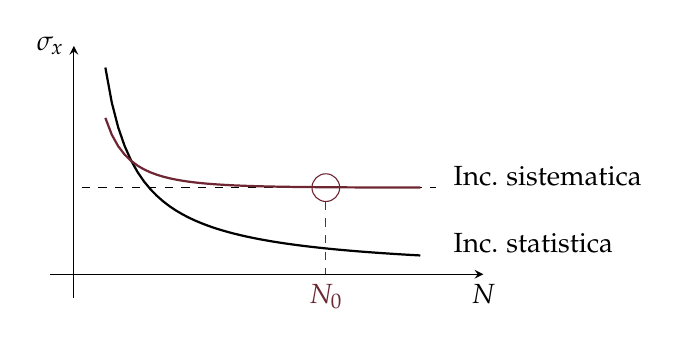
\begin{tikzpicture}[>=stealth]
  \draw[->] (-0.3,0) -- (5.2,0) node[below] {$N$};
  \draw[->] (0,-0.3) -- (0,2.9) node[left] {$\sigma_x$};
  \draw[dashed] (0.1,1.1) -- (4.6,1.1);
  \draw[thick,domain=0.4:4.4,samples=50] plot (\x,{1.05/\x});
  \draw[thick,cteo,domain=0.4:4.4,samples=50] plot (\x,{1.1+0.55*exp(-1.1*\x)/\x});
  \draw[cteo] (3.2,1.1) circle (5pt);
  \draw[cteo,dashed] (3.2,0.92) -- (3.2,0);
  \node[below,cteo] at (3.2,0) {$N_0$};
  \node[right] at (4.7,1.25) {Inc.\ sistematica};
  \node[right] at (4.7,0.4) {Inc.\ statistica};
\end{tikzpicture}
\end{center}
$N_0$: a che $N$ fermarsi per non incorrere nell'errore sistematico

% ------------------------------------------------------------
\section{Precisione e accuratezza}
\lezione{16/09/26}

\chiave{Accuratezza} \fr\ \chiave{Accordo tra} valore della misura $x$ \chiave{e} il misurando $\hat{x}$

\chiave{Precisione} \fr\ \chiave{Consistenza} tra \chiave{misure successive} in stesse condizioni

\chiave{Istogramma}:
\begin{center}
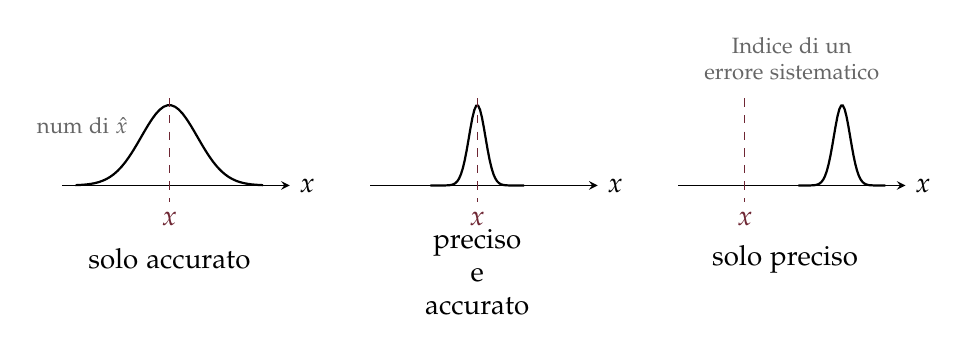
\begin{tikzpicture}[>=stealth,scale=0.85]
  \begin{scope}
    \draw[->] (-1.6,0) -- (1.8,0) node[right] {$x$};
    \draw[thick,domain=-1.4:1.4,samples=50] plot (\x,{1.2*exp(-(\x*\x)/0.35)});
    \draw[cteo,dashed] (0,1.3) -- (0,-0.25) node[below] {$x$};
    \node[grigio,font=\footnotesize] at (-1.3,0.9) {num di $\hat{x}$};
    \node at (0,-1.1) {solo accurato};
  \end{scope}
  \begin{scope}[xshift=4.6cm]
    \draw[->] (-1.6,0) -- (1.8,0) node[right] {$x$};
    \draw[thick,domain=-0.7:0.7,samples=50] plot (\x,{1.2*exp(-(\x*\x)/0.03)});
    \draw[cteo,dashed] (0,1.3) -- (0,-0.25) node[below] {$x$};
    \node[align=center] at (0,-1.3) {preciso\\e\\accurato};
  \end{scope}
  \begin{scope}[xshift=9.2cm]
    \draw[->] (-1.6,0) -- (1.8,0) node[right] {$x$};
    \draw[thick,domain=0.2:1.5,samples=50] plot (\x,{1.2*exp(-((\x-0.85)*(\x-0.85))/0.03)});
    \draw[cteo,dashed] (-0.6,1.3) -- (-0.6,-0.25) node[below] {$x$};
    \node[grigio,font=\footnotesize,align=center] at (0.1,1.9) {Indice di un\\errore sistematico};
    \node at (0,-1.1) {solo preciso};
  \end{scope}
\end{tikzpicture}
\end{center}

\begin{esercizio}{pendolo}{}
\leavevmode\par
\begin{minipage}[c]{0.3\linewidth}
\[
  \begin{aligned}
    T_1 &= 1{,}24\ \mathrm{s} \\
    T_2 &= 1{,}21\ \mathrm{s} \\
    T_3 &= 1{,}34\ \mathrm{s} \\
    T_4 &= 1{,}44\ \mathrm{s} \\
    T_5 &= 1{,}28\ \mathrm{s}
  \end{aligned}
\]
\end{minipage}\hfill
\begin{minipage}[c]{0.6\linewidth}
\[
  \hat{T} = \frac{1}{5} \sum_{i=1}^{5} T_i = 1{,}302\ \mathrm{s}
\]
\[
  \sigma_T = 0{,}02245\ \mathrm{s}
\]
\end{minipage}
\[
  T = (1{,}302 \pm 0{,}022)\ \mathrm{s}
\]
strumento = cronometro $+$ operatore

sensibilità: \quad cronometro \fr\ $0{,}01\ \mathrm{s}$ \qquad operatore \fr\ ?

$T_{\text{vero}} = 1.5$ \fr\ La misura fatta è precisa ma non accurata

Come riduco l'impatto dell'operatore \fr\ errore sistematico

Si prende 10 periodi
\[
  \tau = 10\,T \qquad
  \left.
  \begin{aligned}
    \tau_1 &= \ldots \\
    \tau_2 &= \ldots \\
    \tau_3 &= \ldots
  \end{aligned}
  \right\}
  \quad T = \frac{\tau}{10} \ \Rightarrow\ T = \hat{T} \pm \sigma_T
\]
\end{esercizio}

\begin{attenzione}[NB!]
Se la dispersione è non nulla si può abbattere $\sigma_x$ aumentando $N$ \fr\ A prescindere dallo strumento

Posso andare sotto la sensibilità
\end{attenzione}

Per passare da $\sigma_{T_1} = 0.02$ a $\sigma_{T_2} = 0.001$
\[
  \sigma_T \propto \frac{1}{\sqrt{N}}
\]
\[
  \begin{aligned}
    \sigma_{T_1} &\propto \frac{1}{\sqrt{N_1}} \\
    \sigma_{T_2} &\propto \frac{1}{\sqrt{N_2}}
  \end{aligned}
  \qquad\qquad
  \frac{\sigma_{T_2}}{\sigma_{T_1}} \propto \sqrt{\frac{N_1}{N_2}}
  \ \to\
  \frac{0.001}{0.02} = \left( \sqrt{\frac{N_1}{N_2}} \right)^{2} = \underbrace{\left( \frac{1}{20} \right)^{2}}_{\frac{1}{400}}
\]
\[
  N_2 = N_1 \cdot 400 = 2000 \qquad (N_1 = 5)
\]

% ------------------------------------------------------------
\section{Propagazione dell'incertezza}

\begin{minipage}[c]{0.3\linewidth}
\centering
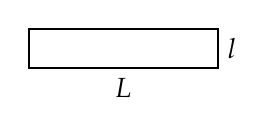
\begin{tikzpicture}
  \draw[thick] (0,0) rectangle (2.4,0.5);
  \node[below] at (1.2,0) {$L$};
  \node[right] at (2.4,0.25) {$l$};
\end{tikzpicture}
\end{minipage}\hfill
\begin{minipage}[c]{0.65\linewidth}
\[
  P = 2(L + l) \qquad
  \left.
  \begin{aligned}
    &\hat{l} \pm \sigma_l \\
    &\hat{L} \pm \sigma_L
  \end{aligned}
  \right\}
  \ \hat{P}\,? \quad \sigma_P\,?
\]
\end{minipage}

In generale\ldots
\[
  f(x, y, z) \qquad
  \left.
  \begin{aligned}
    x &= \hat{x} \pm \sigma_x \\
    y &= \hat{y} \pm \sigma_y \\
    z &= \hat{z} \pm \sigma_z
  \end{aligned}
  \right\}
  \quad f = \hat{f} \pm \sigma_f
\]
$x$, $y$, $z$: indipendenti l'una dall'altra

\subsection*{Somma ($S$)}
\[
  S(x, y) = x + y \qquad
  \begin{aligned}
    x &= \hat{x} \pm \Delta x \\
    y &= \hat{y} \pm \Delta y
  \end{aligned}
  \qquad \text{\grigio{(errore massimo)}}
\]
\[
  \hat{S} = \frac{S_{\max} + S_{\min}}{2} \qquad\qquad \Delta S = \frac{S_{\max} - S_{\min}}{2}
\]
$S_{\max}$? \ $S_{\min}$?
\[
  \begin{aligned}
    S_{\max} &= \hat{x} + \Delta x + \hat{y} + \Delta y \\
    S_{\min} &= \hat{x} - \Delta x + \hat{y} - \Delta y
  \end{aligned}
\]
\grigio{Misurando:}
\[
  \hat{S} = \frac{\hat{x} + \cancel{\Delta x} + \hat{y} + \cancel{\Delta y} + \hat{x} - \cancel{\Delta x} + \hat{y} - \cancel{\Delta y}}{2} = \frac{2\hat{x} + 2\hat{y}}{2} = \hat{x} + \hat{y}
\]
\grigio{Errore massimo:}
\[
  \Delta S = \frac{\cancel{\hat{x}} + \Delta x + \cancel{\hat{y}} + \Delta y - \cancel{\hat{x}} + \Delta x - \cancel{\hat{y}} + \Delta y}{2} = \Delta x + \Delta y
\]
Incert.\ Statistica:
\begin{formulabox}
\[
  \sigma_S = \sqrt{\sigma_x^2 + \sigma_y^2}
\]
\end{formulabox}

\begin{spunto}
Come deduco l'incertezza statistica?

Poiché $x$ e $y$ sono variabili indipenti quindi $\mathrm{Cov}(x, y) = 0$ \grigio{(covarianza)} $\Rightarrow$ si sommano in quadratura
\end{spunto}

\subsection*{Differenza ($D$)}
\[
  \hat{D} = \hat{x} - \hat{y} \qquad\qquad \Delta D = \Delta x + \Delta y
\]
\[
  \begin{aligned}
    D_{\max} &= \hat{x} + \Delta x - (\hat{y} - \Delta y) \\
    D_{\min} &= \hat{x} - \Delta x - (\hat{y} + \Delta y)
  \end{aligned}
\]
\[
  \hat{D} = \frac{\hat{x} + \cancel{\Delta x} - \hat{y} + \cancel{\Delta y} + \hat{x} - \cancel{\Delta x} - \hat{y} - \cancel{\Delta y}}{2} = \hat{x} - \hat{y}
\]
\[
  \Delta D = \frac{\cancel{\hat{x}} + \Delta x - \cancel{\hat{y}} + \Delta y - \cancel{\hat{x}} + \Delta x + \cancel{\hat{y}} + \Delta y}{2} = \Delta x + \Delta y
\]
Incertezza statistica:
\begin{formulabox}
\[
  \sigma_D = \sqrt{\sigma_x^2 + \sigma_y^2}
\]
\end{formulabox}

\subsection*{Prodotto ($P$)}
\[
  \begin{aligned}
    P_{\max} &= (\hat{x} + \Delta x)(\hat{y} + \Delta y) = \hat{x}\hat{y} + \hat{x}\Delta y + \hat{y}\Delta x + \Delta x \Delta y \\
    P_{\min} &= (\hat{x} - \Delta x)(\hat{y} - \Delta y) = \hat{x}\hat{y} - \hat{x}\Delta y - \hat{y}\Delta x + \Delta x \Delta y
  \end{aligned}
\]
\[
  \hat{P} = \frac{P_{\max} + P_{\min}}{2} = \hat{x} \cdot \hat{y} + \Delta x \Delta y \simeq \hat{x}\hat{y}
  \qquad \text{se } \Delta x \ll \hat{x} \text{ e } \Delta y \ll \hat{y}
\]
\[
  \Delta P = \frac{P_{\max} - P_{\min}}{2} = \abs{\hat{x}} \Delta y + \abs{\hat{y}} \Delta x
\]
\grigio{$\abs{\hat{x}}$: se $x$ negativo non va bene perché potrei ottenere $0$ per le fluttuazioni}

\grigio{$\sigma_P$?}

\subsection*{Quoziente ($Q$)}
\[
  Q_{\max} = \frac{\hat{x} + \Delta x}{\hat{y} - \Delta y} \qquad\qquad
  Q_{\min} = \frac{\hat{x} - \Delta x}{\hat{y} + \Delta y}
\]
\[
  \hat{Q} \simeq \frac{\hat{x}}{\hat{y}}
\]
\[
  \Delta Q = \frac{\abs{\hat{x}} \Delta y + \abs{\hat{y}} \Delta x}{\hat{y}^2}
\]
\grigio{$\sigma_Q$?}

\subsection*{Inc.\ Statistica Prod.\ e Quoz.}
Errore relativo: \quad $x = \hat{x} \pm \Delta x$ \qquad $\dfrac{\sigma_x}{\abs{\hat{x}}}$
\begin{formulabox}
\[
  \frac{\sigma_P}{\abs{\hat{P}}} = \frac{\sigma_Q}{\abs{\hat{Q}}} = \sqrt{\left( \frac{\sigma_x}{\abs{\hat{x}}} \right)^2 + \left( \frac{\sigma_y}{\abs{\hat{y}}} \right)^2}
\]
\end{formulabox}

\subsection*{Prodotto per una costante}
\[
  f(x) = c \cdot x \ \to\ \hat{f} = c\,\hat{x} \qquad\qquad \sigma_f = c\,\sigma_x
\]

% ------------------------------------------------------------
\newpage
\section{Sviluppo serie di Taylor}
\lezione{21/9/26}

\begin{definizione}{Serie di Taylor}{serietaylor}
\newline $f(x)$ \grigio{ragionevole (continua e derivabile)} \newline \qquad per $x \to x_0$
\[
  f(x) = \sum_{k=0}^{\infty} \frac{1}{k!} \left. \frac{d^k}{dx^k} f(x) \right|_{x = x_0} (x - x_0)^k
\]
\end{definizione}

\begin{nota}
Nei calcoli di laboratori si usa spesso lo sviluppo di Taylor per approssimare funzioni complicate con polinomi più semplici. In particolare, si considera solo un numero finito di termini della serie, a seconda della precisione richiesta.
\newline\newline
D'altronde di solito il numero di passaggi considerati, per le esperienze che condurremo in laboratorio, è $k=2$
\end{nota}

\[
  k = 2 \ \to\ f(x) = f(x_0) + \left. \frac{d}{dx} f(x) \right|_{x = x_0} (x - x_0) + \frac{1}{2} \left. \frac{d^2}{dx^2} f(x) \right|_{x = x_0} (x - x_0)^2 + \ldots
\]
\grigio{$\big|_{x = x_0}$: calcolata in}

$k = 1$
\begin{center}
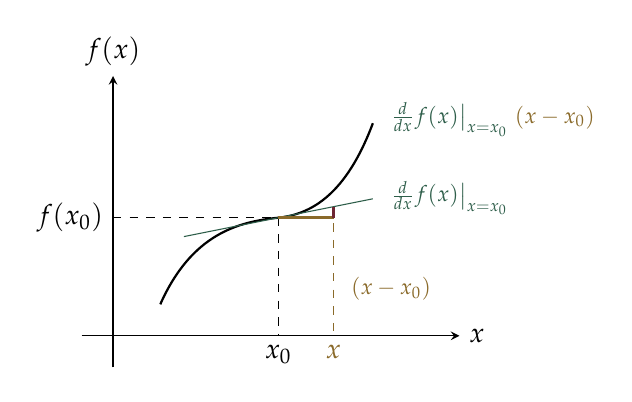
\begin{tikzpicture}[>=stealth]
  \draw[->] (-0.4,0) -- (4.4,0) node[right] {$x$};
  \draw[->] (0,-0.4) -- (0,3.3) node[above] {$f(x)$};
  \draw[thick] (0.6,0.4) .. controls (1.0,1.3) and (1.6,1.45) .. (2.1,1.5) .. controls (2.6,1.55) and (3.0,1.9) .. (3.3,2.7);
  \draw[cese] (0.9,1.26) -- (3.3,1.74);
  \draw[dashed] (0,1.5) node[left] {$f(x_0)$} -- (2.1,1.5);
  \draw[dashed] (2.1,1.5) -- (2.1,0) node[below] {$x_0$};
  \draw[dashed,coss] (2.8,1.64) -- (2.8,0) node[below] {$x$};
  \draw[very thick,coss] (2.1,1.5) -- (2.8,1.5);
  \draw[very thick,cteo] (2.8,1.5) -- (2.8,1.64);
  \node[right,coss,font=\footnotesize] at (2.9,0.6) {$(x - x_0)$};
  \node[right,cese,font=\footnotesize] at (3.4,1.75) {$\frac{d}{dx} f(x)\big|_{x = x_0}$};
  \node[right,font=\footnotesize] at (3.4,2.75) {{\color{cese}$\frac{d}{dx} f(x)\big|_{x = x_0}$} {\color{coss}$(x - x_0)$}};
\end{tikzpicture}
\end{center}

\begin{esempio}{}{}
\[
  f(x) = (1 + x)^{\alpha} \qquad x_0 = 0
\]
Serie di Taylor:
\[
  f(x) \simeq f(0) + \left. \alpha (1 + x)^{\alpha - 1} \right|_{x = 0} \cdot (x - 0) \simeq 1 + \alpha x \qquad \text{se } x \to x_0
\]
\end{esempio}

% ------------------------------------------------------------
\newpage
\section{Propagazione dell'errore nella funzione}

Applicazione
\[
  \frac{1}{1.05} = (1 + 0.05)^{-1} \simeq 1 + (-1)\,0.05 = 1 - 0.05 = 0.95
\]
Ci può essere utile per fare conti analiticamente

\subsection*{Errore massimo}
\[
  x = \hat{x} \pm \Delta x
\]
\begin{minipage}[c]{0.45\linewidth}
\centering
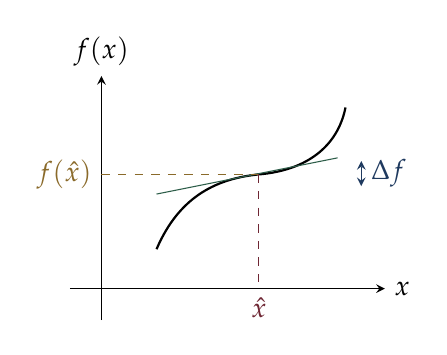
\begin{tikzpicture}[>=stealth]
  \draw[->] (-0.4,0) -- (3.6,0) node[right] {$x$};
  \draw[->] (0,-0.4) -- (0,2.7) node[above] {$f(x)$};
  \draw[thick] (0.7,0.5) .. controls (1.0,1.2) and (1.5,1.4) .. (2.0,1.45) .. controls (2.6,1.5) and (3.0,1.8) .. (3.1,2.3);
  \draw[cese] (0.7,1.2) -- (3.0,1.66);
  \draw[dashed,coss] (0,1.45) node[left] {$f(\hat{x})$} -- (2.0,1.45);
  \draw[dashed,cteo] (2.0,1.45) -- (2.0,0) node[below] {$\hat{x}$};
  \draw[<->,cdef] (3.3,1.3) -- (3.3,1.62) node[midway,right] {$\Delta f$};
\end{tikzpicture}
\end{minipage}\hfill
\begin{minipage}[c]{0.5\linewidth}
Se $x$ è un intervallo, anche $f(x)$ lo è, ma quale?
\[
  \Delta f = \left| \frac{d}{dx} f \right| \Delta x
\]
\end{minipage}
\begin{formulabox}
\[
  f(\hat{x}) = f(x_0) \pm \underbrace{\left| \left. \frac{d}{dx} f(x) \right|_{\hat{x}} \right| \Delta x}_{\Delta f}
\]
\end{formulabox}
Se $f' = 0$ allora si fa $(f')''$ finché non diventa $\neq 0$

\subsection*{Errore statistico}
\begin{formulabox}
\[
  f(x) = f(\hat{x}) \pm \left| \left. \frac{\partial}{\partial x} f(x) \right|_{\hat{x}} \right| \sigma_x
\]
\end{formulabox}

\subsection*{In 3 variabili}
\[
  f(x, y, z) \qquad
  \begin{aligned}
    x &= \hat{x} \pm \sigma_x \\
    y &= \hat{y} \pm \sigma_y \\
    z &= \hat{z} \pm \sigma_z
  \end{aligned}
\]
\chiave{Sommo in quadratura le varie incertezze}
\begin{formulabox}
\begin{multline*}
  \sigma_f^2 = \left( \left. \frac{\partial}{\partial x} f(x, y, z) \right|_{\hat{x}, \hat{y}, \hat{z}} \right)^{2} \cdot \sigma_x^2
  + \left( \left. \frac{\partial}{\partial x} f(x, y, z) \right|_{\hat{x}, \hat{y}, \hat{z}} \right)^{2} \sigma_y^2 + {} \\
  + \left( \left. \frac{\partial}{\partial x} f(x, y, z) \right|_{\hat{x}, \hat{y}, \hat{z}} \right)^{2} \sigma_z^2
\end{multline*}
\end{formulabox}

\begin{attenzione}
\chiave{Funziona se $x$, $y$, $z$ indipendenti!}
\end{attenzione}

\chiave{$\partial$: derivata parziale} \fr\ considero una costante tutto ciò che non varia

es.\quad $f(x) = x y$ \qquad $\dfrac{\partial}{\partial x} f(x) = y$ \quad \grigio{($y$ considerata costante)}

es.\quad $f(x) = x + y$ \qquad $\dfrac{\partial}{\partial x} f(x) = 1$

\[
  G(x, y, z) = x^{\alpha} y^{\beta} z^{\gamma}
\]
\[
  \begin{aligned}
    \frac{\partial}{\partial x} G &= \alpha x^{\alpha - 1} \cdot y^{\beta} \cdot z^{\gamma} = \frac{\alpha G}{x} \\[4pt]
    \frac{\partial}{\partial y} G &= \beta y^{\beta - 1} \cdot x^{\alpha} \cdot z^{\gamma} = \frac{\beta G}{y} \\[4pt]
    \frac{\partial}{\partial z} G &= \gamma z^{\gamma - 1} \cdot x^{\alpha} \cdot y^{\beta} = \frac{\gamma G}{z}
  \end{aligned}
\]
\[
  \begin{aligned}
    \sigma_G^2 &= \left( \left. \frac{\partial G}{\partial x} \right|_{\ldots} \sigma_x \right)^{2} + \ldots \\
    &= \left( \frac{\alpha G}{x}\, \sigma_x \right)^{2} + \left( \frac{\beta G}{y}\, \sigma_y \right)^{2} + \left( \frac{\gamma G}{z}\, \sigma_z \right)^{2} \\
    &= G^2 \left[ \left( \alpha\, \frac{\sigma_x}{x} \right)^{2} + \left( \beta\, \frac{\sigma_y}{y} \right)^{2} + \left( \gamma\, \frac{\sigma_z}{z} \right)^{2} \right]
  \end{aligned}
\]
$\dfrac{\sigma_x}{x}$, $\dfrac{\sigma_y}{y}$, $\dfrac{\sigma_z}{z}$: \underline{errore relativo}
\begin{formulabox}
\[
  \left( \frac{\sigma_G}{G} \right)^{2} = \left( \frac{\alpha\, \sigma_x}{x} \right)^{2} + \left( \frac{\beta\, \sigma_y}{y} \right)^{2} + \left( \frac{\gamma\, \sigma_z}{z} \right)^{2}
\]
\end{formulabox}
$\dfrac{\sigma_G}{G}$: \chiave{errore relativo di $G$}

\begin{esempio}{}{}
\[
  f(x) = x^2 \qquad\qquad \sqrt{\sigma_f^2} = \sqrt{(2 \hat{x} \cdot \sigma_x)^2} \qquad \text{Giusto}
\]
\end{esempio}

% ------------------------------------------------------------
\section{Compatibilità tra misure}

\subsection*{Errore massimo}
\begin{minipage}[c]{0.32\linewidth}
\[
  \begin{aligned}
    x_1 &= \hat{x}_1 \pm \Delta x_1 \\
    x_2 &= \hat{x}_2 \pm \Delta x_2
  \end{aligned}
\]
\end{minipage}\hfill
\begin{minipage}[c]{0.62\linewidth}
\centering
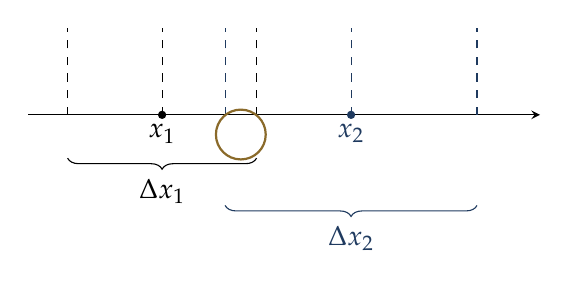
\begin{tikzpicture}[>=stealth]
  \draw[->] (-0.5,0) -- (6,0);
  \fill (1.2,0) circle (1.5pt) node[below] {$x_1$};
  \fill[cdef] (3.6,0) circle (1.5pt) node[below] {$x_2$};
  \foreach \x in {0,2.4} \draw[dashed] (\x,0) -- (\x,1.1);
  \draw[dashed] (1.2,0) -- (1.2,1.1);
  \foreach \x in {2.0,5.2} \draw[dashed,cdef] (\x,0) -- (\x,1.1);
  \draw[dashed,cdef] (3.6,0) -- (3.6,1.1);
  \draw[decorate,decoration={brace,mirror,amplitude=4pt}] (0,-0.55) -- (2.4,-0.55) node[midway,below=4pt] {$\Delta x_1$};
  \draw[cdef,decorate,decoration={brace,mirror,amplitude=4pt}] (2.0,-1.15) -- (5.2,-1.15) node[midway,below=4pt] {$\Delta x_2$};
  \draw[coss,thick] (2.2,-0.25) circle (9pt);
\end{tikzpicture}
\end{minipage}

Se la misura è sicuramente dentro $\Delta x_1$ e $\Delta x_2$.

Allora \fr\ nell'intersezione c'è $x$
\begin{formulabox}
\[
  \text{Se:}\quad \abs{\hat{x}_1 - \hat{x}_2} \leq \Delta x_1 + \Delta x_2 \ \Rightarrow\ \text{\chiave{misure compatibili}}
\]
\end{formulabox}
\grigio{NB! Le misure non sono uguali, sono \fr\ compatibili!}

\subsection*{Errore statistico}
\begin{formulabox}
\[
  \abs{\hat{x}_1 - \hat{x}_2} \leq (2 \text{ o } 3)\, \sqrt{\sigma_{x_1}^2 + \sigma_{x_2}^2} \ \Rightarrow\ \text{\chiave{misura compatibile}}
\]
\end{formulabox}
Serve un coefficiente perché \chiave{l'err.\ stat.\ non ha il $100\%$ di contenere $x$}

Che numero \fr\ $2/3$

\begin{spunto}
NB! In incertezza statistica si \chiave{somma in quadratura}
\end{spunto}

% ------------------------------------------------------------
\section{Approssimazione}

Relazione d'ordine \fr\ $x$ più grande/piccolo di $y$

$x > y$ \fr\ NON si può dire

Ma\ldots
\[
  \left.
  \begin{aligned}
    &x \gg y \ \text{ se } \ x \geq 10\,y && \text{\grigio{($8$, $9$, $10$ vanno bene)}} \\[4pt]
    &x \ll y \ \text{ se } \ x \leq \frac{1}{10}\,y && \text{\grigio{($\tfrac{1}{8}$, $\tfrac{1}{9}$, $\tfrac{1}{10}$ vanno bene)}}
  \end{aligned}
  \right\}
  \ \text{Almeno possiamo semplificarli}
\]

\subsection*{Pendolo \fr\ Approssimazione piccole oscillazioni}
\begin{minipage}[c]{0.6\linewidth}
\[
  \ddot{\theta} + \omega_0^2 \sin\theta = 0
\]
\end{minipage}\hfill
\begin{minipage}[c]{0.3\linewidth}
\centering
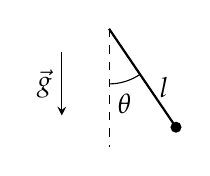
\begin{tikzpicture}[>=stealth]
  \draw[dashed] (0,0) -- (0,-1.5);
  \draw[thick] (0,0) -- (0.85,-1.25) node[pos=0.6,right] {$l$};
  \fill (0.85,-1.25) circle (2pt);
  \draw (0,-0.7) arc (-90:-55.8:0.7);
  \node at (0.2,-0.95) {$\theta$};
  \draw[->] (-0.6,-0.3) -- (-0.6,-1.1) node[midway,left] {$\vec{g}$};
\end{tikzpicture}
\end{minipage}

\giu\ $\theta = \theta(t)$: Non c'è soluzione analitica per \underline{qualsiasi $\theta$}

Ma per $\theta$ piccoli $\sin\theta \simeq \theta$ \quad Sviluppo di Taylor
\[
  T = 2\pi \sqrt{\frac{l}{g}}\, \underbrace{\left( 1 + \theta_0^2\, \frac{1}{16} + \frac{11}{3072}\, \theta_0^4 + \ldots \right)}_{\text{\grigio{Sviluppo di Taylor}}}
\]
$\cancel{\theta \ll 1}$ in laboratorio non va bene perché misuro $T$ con una incertezza
\[
  T(\theta_0) = T_0 \left( 1 + \frac{\theta_0^2}{16} + \ldots \right)
  \qquad\qquad
  T = 2\pi \sqrt{\frac{l}{g}} \ \bigr\}\ \text{se } \sin\theta \simeq \theta
\]
$\dfrac{\theta_0^2}{16}$ \fr\ posso trascurarlo, quindi posso approssimare $T(\theta_0) \simeq T_0$?

Se non ne risento nella mia misura \fr\ SI

Dunque confronto es.\ \fr\ $T_0\, \dfrac{\theta^2}{16}$ con $\sigma_T$ e capisco

Dunque non posso saperlo a priori:
\[
  \begin{cases}
    \text{Se } \sigma_T \gg T_0\, \dfrac{\theta}{16} \text{ allora: Trascuro } T_0\, \dfrac{\theta}{16} \ \to\ \text{Piccole oscillazioni} \\[8pt]
    \text{Sennò\ldots\ NON posso trascurarlo}
  \end{cases}
\]
\[
  \text{\grigio{$\theta \ll \sqrt{16\, \dfrac{\sigma_T}{T_0}} = 4 \sqrt{\dfrac{\sigma_T}{T_0}} = \theta_{\max}$}}
\]
Definizione operativa di piccole oscillazioni

\begin{attenzione}[NB!]
Se non influisce nella mia misura \fr\ lo posso trascurare
\end{attenzione}

\begin{spunto}
NB! Se uso la formula es.\ $T = 2\pi \sqrt{\dfrac{l}{g}}$ ma l'incertezza mi ``chiede'' di usare Taylor. E ricalcolo $g$ \fr\ $g$ è errata: \chiave{errore sistematico} che non si riduce con $N$ misure
\end{spunto}

% ------------------------------------------------------------
\newpage
\section{Errore sistematico}

Da cosa dipende?
\begin{itemize}[label=--]
  \item Dall'esperimento
\end{itemize}

\begin{enumerate}[label=\protect\cerchio{\arabic*}]
  \item \chiave{Strumenti di misura}
  \begin{itemize}[label=\fr]
    \item Uso improprio (lettura sbagliata)
    \item Problemi di calibrazione degli strumenti
  \end{itemize}
  \begin{center}
  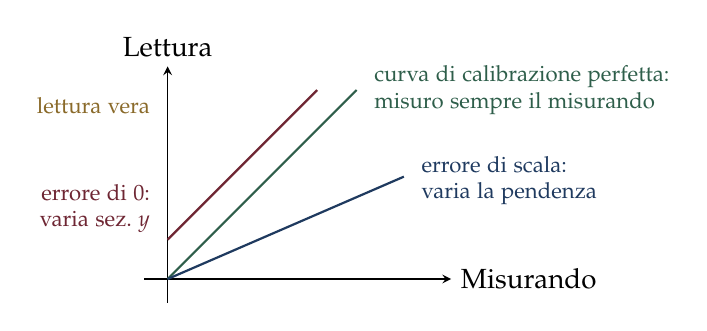
\begin{tikzpicture}[>=stealth]
    \draw[->] (-0.3,0) -- (3.6,0) node[right] {Misurando};
    \draw[->] (0,-0.3) -- (0,2.7) node[above] {Lettura};
    \draw[thick,cese] (0,0) -- (2.4,2.4);
    \draw[thick,cteo] (0,0.5) -- (1.9,2.4);
    \draw[thick,cdef] (0,0) -- (3.0,1.3);
    \node[right,cese,align=left,font=\footnotesize] at (2.5,2.4) {curva di calibrazione perfetta:\\misuro sempre il misurando};
    \node[left,cteo,align=right,font=\footnotesize] at (-0.1,0.9) {errore di $0$:\\varia sez.\ $y$};
    \node[right,cdef,align=left,font=\footnotesize] at (3.1,1.25) {errore di scala:\\varia la pendenza};
    \node[left,coss,font=\footnotesize] at (-0.1,2.2) {lettura vera};
  \end{tikzpicture}
  \end{center}
  \grigio{Errore di scala, es.: dilatazione termica dello strumento}

  \item \chiave{Fattori esterni} (o ambientali)
  \item \chiave{Incertezze di modellizzazione} \fr\ Modello inadeguato per ciò che misuro \grigio{(es.\ pendolo prima)}
\end{enumerate}

Per rimediare a questi errori \fr\ Si verifica la presenza di errori più noti
\begin{itemize}[label=\fr]
  \item Con strumenti più precisi
  \item Facendo misure note \fr\ vari punti di calibrazione
\end{itemize}

% ------------------------------------------------------------
\newpage
\section{Rappresentare i dati}

\begin{attenzione}[NB!]
Tutto deve essere descritto e leggibile
\end{attenzione}

\subsection*{Tabella}
\begin{minipage}[c]{0.5\linewidth}
\centering
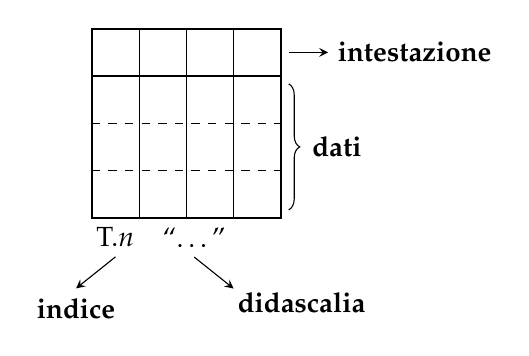
\begin{tikzpicture}[>=stealth]
  \draw[thick] (0,0) rectangle (2.4,2.4);
  \draw[thick] (0,1.8) -- (2.4,1.8);
  \foreach \x in {0.6,1.2,1.8} \draw (\x,0) -- (\x,2.4);
  \foreach \y in {0.6,1.2} \draw[dashed] (0,\y) -- (2.4,\y);
  \draw[->] (2.5,2.1) -- (3.0,2.1) node[right] {\chiave{intestazione}};
  \draw[decorate,decoration={brace,amplitude=4pt}] (2.5,1.7) -- (2.5,0.1) node[midway,right=5pt] {\chiave{dati}};
  \node[below] (tn) at (0.3,0) {T.$n$};
  \node[below] (did) at (1.3,0) {``\ldots''};
  \draw[->] (tn.south) -- ++(-0.5,-0.4) node[below] {\chiave{indice}};
  \draw[->] (did.south) -- ++(0.5,-0.4) node[below right=-2pt] {\chiave{didascalia}};
\end{tikzpicture}
\end{minipage}\hfill
\begin{minipage}[c]{0.45\linewidth}
\chiave{Incertezze}? se tutte uguali in didascalia, sennò con i dati
\end{minipage}

\subsection*{Istogramma}
\fr\ quante volte occorre una misura

\giu\ \chiave{distribuzione delle misure}

\begin{minipage}[c]{0.5\linewidth}
\centering
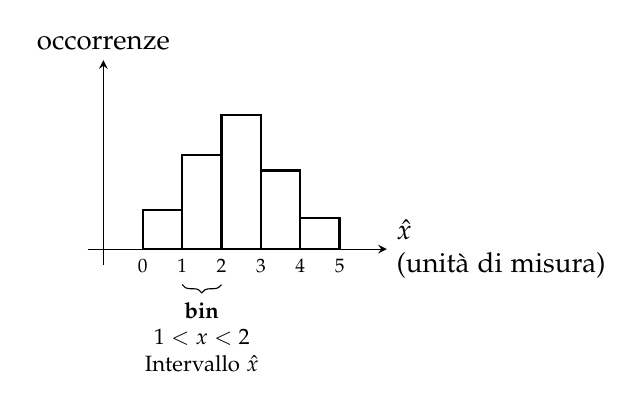
\begin{tikzpicture}[>=stealth]
  \draw[->] (-0.2,0) -- (3.6,0) node[right,align=left] {$\hat{x}$\\(unità di misura)};
  \draw[->] (0,-0.2) -- (0,2.4) node[above] {occorrenze};
  \foreach \x/\h in {0.5/0.5,1.0/1.2,1.5/1.7,2.0/1.0,2.5/0.4}
    \draw[thick] (\x,0) rectangle (\x+0.5,\h);
  \foreach \x/\l in {0.5/0,1.0/1,1.5/2,2.0/3,2.5/4,3.0/5} \node[below,font=\scriptsize] at (\x,0) {\l};
  \draw[decorate,decoration={brace,mirror,amplitude=3pt}] (1.0,-0.45) -- (1.5,-0.45) node[midway,below=3pt,font=\footnotesize,align=center] {\chiave{bin}\\$1 < x < 2$\\Intervallo $\hat{x}$};
\end{tikzpicture}
\end{minipage}\hfill
\begin{minipage}[c]{0.45\linewidth}
Dobbiamo tenere di conto:
\begin{itemize}[label=\fr]
  \item Min
  \item Max
\end{itemize}
\begin{itemize}[label=--]
  \item \#bin
  \item larghezza bin rispetto all'incertezza
\end{itemize}
\end{minipage}

\begin{spunto}
Da rivedere a modo \fr\ soprattutto nella pratica
\end{spunto}

\subsection*{Grafico di dispersione}
\begin{minipage}[c]{0.5\linewidth}
\centering
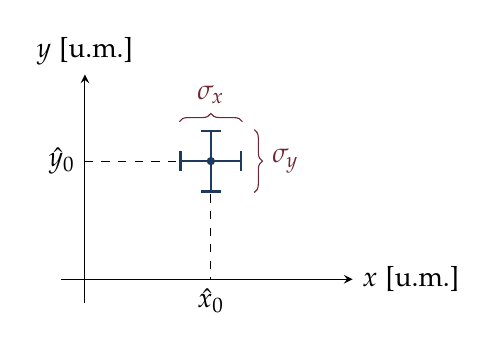
\begin{tikzpicture}[>=stealth]
  \draw[->] (-0.3,0) -- (3.4,0) node[right] {$x$ [u.m.]};
  \draw[->] (0,-0.3) -- (0,2.6) node[above] {$y$ [u.m.]};
  \draw[dashed] (0,1.5) node[left] {$\hat{y}_0$} -- (1.6,1.5);
  \draw[dashed] (1.6,1.5) -- (1.6,0) node[below] {$\hat{x}_0$};
  \draw[thick,cdef,|-|] (1.2,1.5) -- (2.0,1.5);
  \draw[thick,cdef,|-|] (1.6,1.1) -- (1.6,1.9);
  \fill[cdef] (1.6,1.5) circle (1.5pt);
  \draw[cteo,decorate,decoration={brace,amplitude=3pt}] (1.2,2.0) -- (2.0,2.0) node[midway,above=3pt] {$\sigma_x$};
  \draw[cteo,decorate,decoration={brace,amplitude=3pt}] (2.15,1.9) -- (2.15,1.1) node[midway,right=3pt] {$\sigma_y$};
\end{tikzpicture}
\end{minipage}\hfill
\begin{minipage}[c]{0.45\linewidth}
\chiave{Si usa per testare un modello}
\end{minipage}

\subsection*{Fit}
\begin{esempio}{moto rettilineo uniforme}{}
\leavevmode\par
\begin{minipage}[c]{0.4\linewidth}
\[
  x(t) = x_0 + v_0 t
\]
\[
  v_0 = \frac{\Delta x}{\Delta t}
\]
\end{minipage}\hfill
\begin{minipage}[c]{0.55\linewidth}
\centering
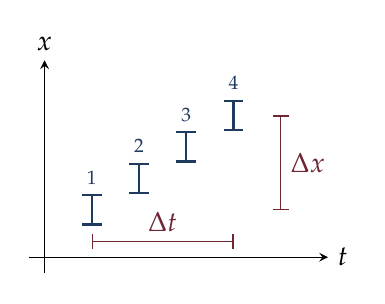
\begin{tikzpicture}[>=stealth]
  \draw[->] (-0.2,0) -- (3.6,0) node[right] {$t$};
  \draw[->] (0,-0.2) -- (0,2.5) node[above] {$x$};
  \foreach \t/\y/\n in {0.6/0.6/1,1.2/1.0/2,1.8/1.4/3,2.4/1.8/4} {
    \draw[thick,cdef,|-|] (\t,\y-0.2) -- (\t,\y+0.2);
    \node[above,cdef,font=\scriptsize] at (\t,\y+0.2) {\n};
  }
  \draw[cteo,|-|] (0.6,0.2) -- (2.4,0.2) node[midway,above] {$\Delta t$};
  \draw[cteo,|-|] (3.0,0.6) -- (3.0,1.8) node[midway,right] {$\Delta x$};
\end{tikzpicture}
\end{minipage}
\[
  x_i \pm \sigma_i \qquad\qquad \Delta x = x_4 - x_1 \qquad\qquad \sigma_{\Delta x} = \sqrt{\sigma^2 + \sigma^2} = \sqrt{2}\, \sigma
\]
\grigio{($x_4$, $x_1$: incertezze uguali)}
\[
  \sigma_v = \frac{1}{\Delta t} \cdot \sigma_{\Delta x} \qquad\qquad v_0 = \frac{\Delta x}{\Delta t} \pm \sigma_v
\]
Ma sto considerando solo due dati?
\end{esempio}

Come posso considerare tutti i dati? = Fitting!

FIT
\begin{itemize}[label=\giu]
  \item \chiave{Input = modello}
  \item \chiave{Input = misure}
  \item \chiave{Output = valore dei parametri del modello che meglio approssimano le misure}

  \fr\ Trovare la curva che più avvicina i dati.
\end{itemize}
Dunque che: \chiave{algoritmo} $\leftarrow$ \chiave{minimizza la distanza tra la curva e i dati}

\chiave{\texttt{scipy.optimize.curve\_fit}}
\begin{itemize}[label=\fr]
  \item Non troppi parametri \fr\ overfit
  \item Non pochi parametri
\end{itemize}

\begin{spunto}
!!! Da rivedere e provare a fare sul codice
\end{spunto}

% ------------------------------------------------------------
\newpage
\section{Decade}

Intervallo: \qquad $10^{n}$
\begin{center}
\begin{tabular}{@{}lll@{}}
  $[\underbrace{0, \ldots, 10}]$ & 1 decade & $10 = 10^{1}$ \quad (esponente \fr\ decadi) \\[10pt]
  $[\underbrace{0, \ldots, 10}, \underbrace{\ldots, 100}]$ & 2 decadi & $100 = 10^{2}$ \quad (esponente \fr\ decadi) \\
\end{tabular}
\end{center}

\chiave{distanza in decadi} tra $x_1$, $x_2$
\begin{formulabox}
\[
  \mathrm{dex}(x_1, x_2) = \log_{10} \left( \frac{x_2}{x_1} \right)
\]
\end{formulabox}

% ------------------------------------------------------------
\section{Scala non lineare}
\subsection*{Scala logaritmica}

\centering
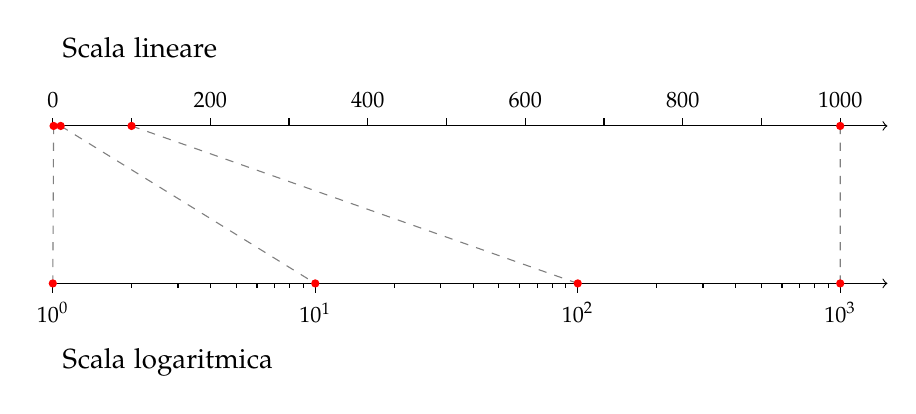
\begin{tikzpicture}
  % --- scala lineare (1 cm = 100 unità) ---
  \node[anchor=west] at (0,3.0) {Scala lineare};
  \draw[->] (0,2) -- (10.6,2);
  \foreach \x in {0,...,10}
    \draw (\x,2) -- (\x,2.1);
  \foreach \x in {0,2,...,10} {
    \pgfmathtruncatemacro{\v}{100*\x}
    \node[above, font=\footnotesize] at (\x,2.1) {\v};
  }

  % --- scala logaritmica (una decade = 10/3 cm) ---
  \node[anchor=west] at (0,-1.0) {Scala logaritmica};
  \draw[->] (0,0) -- (10.6,0);
  \foreach \d in {0,1,2}
    \foreach \m in {2,...,9}
      \draw ({10/3*(\d+log10(\m))},0) -- ({10/3*(\d+log10(\m))},-0.06);
  \foreach \d in {0,...,3}
    \draw ({10/3*\d},0) -- ({10/3*\d},-0.12)
      node[below, font=\footnotesize] {$10^{\d}$};

  % --- stessi valori sulle due scale ---
  \foreach \d in {0,...,3} {
    \draw[dashed, gray] ({10^\d/100},2) -- ({10/3*\d},0);
    \fill[red] ({10^\d/100},2) circle (1.5pt);
    \fill[red] ({10/3*\d},0) circle (1.5pt);
  }
\end{tikzpicture}

In una scala lineare la posizione di un valore $x$ sull'asse è proporzionale
a $x$: a distanze uguali corrispondono \emph{differenze} uguali (ad esempio
tra $100$ e $200$ c'è la stessa distanza che tra $800$ e $900$). In una scala
logaritmica la posizione è invece proporzionale a $\log_{10} x$: a distanze
uguali corrispondono \emph{rapporti} uguali, per cui ogni decade
($1$--$10$, $10$--$100$, $100$--$1000$) occupa la stessa lunghezza. Per
questo motivo le tacche intermedie si addensano verso la fine di ogni decade
e lo zero non è rappresentabile, poiché $\log_{10} 0$ non è definito.

Come mostra la figura~\ref{fig:scale}, la scala logaritmica è utile quando i
dati coprono più ordini di grandezza: su una scala lineare i valori piccoli
sarebbero indistinguibili, mentre su quella logaritmica ogni ordine di
grandezza ha lo stesso peso visivo. Inoltre, in scala logaritmica un
andamento esponenziale (asse $y$ logaritmico) o una legge di potenza
(entrambi gli assi logaritmici) appaiono come una retta.

\end{document}

